\section{Background and Basic Ideas}
\label{section:background}
Formally, we define a flow record as a key-value pair $(key, count)$, 
where $key$ is the ID of the flow, and $count$ is the number of packets belonging to this flow. 
A simple example is like this: the flow ID contains the source and destination IP addresses, 
and packets with exactly the same source and destination belong to the same flow. 
The definition is general, since the flow ID can also be a subnet prefix, a transport layer port, 
or even a keyword embedded in application data. A naive method to maintain flow records is to 
save them in a hash table, but multiple flows may be hashed to the same bucket in the table. 
Mechanisms to resolve collisions in hash tables include classic ones like separate chaining 
and linear probing, and more sophisticated ones like Cuckoo hashing \cite{pagh_cuckoo_2004}.
However, in the worst case, they need unbounded time for insertion or lookup, thus are not 
adequate for our purpose. 

Before presenting HashFlow, we briefly review several recently proposed algorithms,
i.e., HashPipe\cite{sivaraman_heavy-hitter_2017}, ElasticSketch\cite{yang_elastic_2018} and FlowRadar\cite{li_flowradar:_2016}, and try to point out some minor defects in the algorithms. We will assume that the readers are familiar with the algorithms.

HashPipe\cite{sivaraman_heavy-hitter_2017} uses a series of independent hash tables (each with a different hash function). The first table is used to effectively accommodate new flows and evict the existing flows when collision occurs, otherwise new flows will have little chance to stay if large flows accumulate in the table. But on the other hand, this strategy frequently 
splits one flow record into multiple records that are stored in different hash tables, each with a partial count, 
since an existing flow may be evicted but new packets of this flow may still arrive later. 
This effect makes the utilization of memory less efficient, and makes the packet count less accurate. 

In ElasticSketch\cite{yang_elastic_2018}, due to the collisions and eviction strategy employed, a flow record may also be split 
into multiple records, and the packet counter is not accurate. The count-min sketch is introduced to help the flow size 
estimation. However, since the count-min sketch itself may not be accurate, the estimation accuracy is limited,  
which is especially true if the sketch is occupied by too many flows. 


%Unlike HashPipe and ElasticSketch, FlowRadar\cite{li_flowradar:_2016} tries to record all the flows. 
In FlowRadar\cite{li_flowradar:_2016}, flow information is encoded into a flow set, and then we can recover (some) flow IDs and the corresponding packet counts during the post processing phase. However, the chances that such decoding succeeds drop abruptly if the table is heavily loaded and there are not enough flows that don't collide with any other ones.

%FlowRadar records the size of every flow accurately when there is sufficient memory. However, when the value of $\frac{\text{num. of cells in the counting table}}{\text{num. of flows cached}}$ is less than some threshold (about 1.24), the performance of FlowRadar will degrade abruptly and many flows will fail to be decoded. So it is challenging to use it in the real networks where bursty traffic occurs frequently.

%As stated in Section~\ref{section:introduction}, there are two aspects that need to be considered when designing the measurement algorithms: (a) there is a small amount of SRAM (e.g., no more than 10 MB) in network elements that can be used for network measurement. (b) only a small amount of time (e.g., no more than 100 ns) are allowed for measurement algorithms to process a packet while the access time of SRAM is around 1-10 ns. So we aim to minimize the time/space complexity while guaranteeing the performance of the algorithm. First of all, we use hash table as a basic component of HashFlow. In the following we will present the reasoning behind the strategies we take in designing HashFlow.

With these in mind, we then analyze a few tradeoffs and design choices 
for time and space efficient collection of flow records.

1) {\em With limited memory, discard flows when necessary.} Pouring too many flows into a 
hash table or sketch will cause frequent collision, and either increase the processing overhead, 
or decrease the accuracy of the information that can be retrieved. 
For example, FlowRadar faces severe degradation in its decoding capability
 when the number of flows exceeds its capacity 
(this effect and the turning point can be clearly seen in our evaluation, 
for example, Fig. \ref{fig:comparison_concurrent_flows_increases_flow_monitoring} for flow set monitoring 
and Fig. \ref{fig:comparison_concurrent_flows_increases_fs_estimation} for flow size estimation).  
In most situations, network traffic is skewed such that 
only a small portion of elephant flows contain a large number of packets. 
For example, in one campus trace we use, 7.7\% of the flows contribute more than 85\% of the packets. 
It will be better to discard mice flows with few packets than elephant ones, 
since the latter have a greater impact on most applications, 
such as heavy hitter detection, traffic engineering and billing. It is often enough to maintain summarized information for the mice flows.

2) {\em A flow should be consistently stored in one record.} Both HashPipe and ElasticSketch 
may split one flow into multiple fragments stored in different tables. This not only wastes memory, 
but also causes the packet count less accurate, which in turn affects the eviction strategies.  
By storing a flow in a consistent record, we can achieve both better memory utilization and 
higher accuracy. 

3) {\em If better memory utilization can be achieved by trading off a little efficiency, have a try.} 
This is particularly worth to do when network equipment is becoming more ``software-defined'', 
where their functionalities can be  ``programmed'', 
and the additional operations can be easily paralleled or pipelined. 
By the nature of the ball and urn model \cite{urn} of hash tables, 
there will be a few empty buckets of a hash table that have never been used, and the utilization will be improved by feeding more flows into the hash table or hashing a flow multiple times to find a proper bucket. 
Both HashPipe and ElasticSketch propose to split the hash table into multiple small tables and use multiple hash functions to improve the utilization, 
but in different ways. Our collision resolution strategy is more similar to 
that of HashPipe than ElasticSketch. 
Later, we will show our strategy can make an effective use of the table buckets.

\iffalse
\subsection{It is impossible to store every flow with fixed memory.}
There are some sketches such as count-min sketch\cite{cormode_countmin_2005} and counter tree\cite{chen_counter_2017} that can pour any amount of information into it. These sketches are usually taken as a component to design some advanced measurement algorithms. For example, ElasticSketch\cite{yang_elastic_2018} takes a count-min sketch as the light table. The drawback of the type of sketches is that as the number of flows in the sketch increases, the error will be accumulated and the accuracy of the information provided by the sketches will degrade constantly. As an example, we create a count-min sketch with 4 rows and each row consists of 2K cells. We feed a number of flows into the sketch and then query the sketch for the sizes of the flows. Finally we calculate the ARE (Average Relative Error) of the estimated sizes of the flows as defined in Section~\ref{section:evaluation}. Fig.~\ref{fig:countminsketchare} shows that as the number of flows increases from 1K to 10K, the ARE of the estimated flow sizes is increased from 0.02 to 3.66. So if we feed too much information into the data structures like count-min sketch, the accuracy of the query result will be so low that it is nearly unusable. Take this in mind, we will discard the less important information to guarantee the accuracy of the most important information when designing HashFlow.

\begin{figure}
    \centering
    \begin{minipage}{0.24\textwidth}
        \centering
        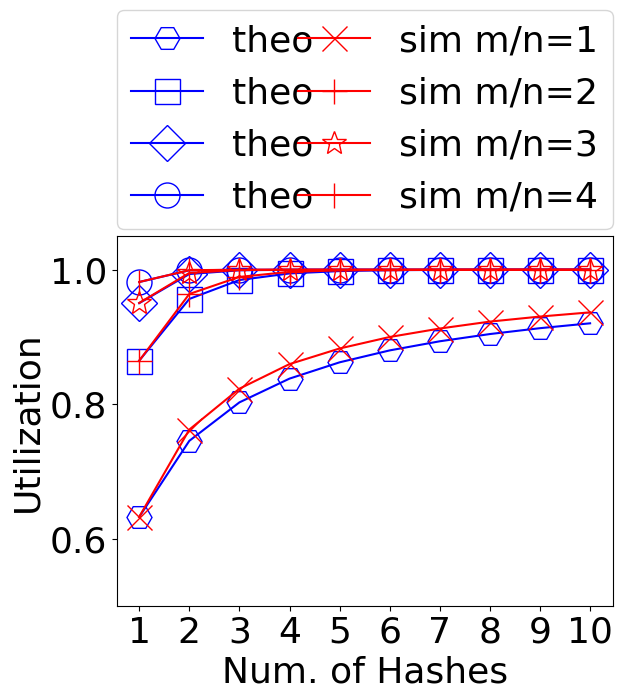
\includegraphics[width=\linewidth]{figures/exp84481/hash_table_utilization}
        \caption{The utilization ratio of the hash table when the number of hashes is increased from 1 to 10.}
        \label{fig:cachehitratio}
    \end{minipage}
    \begin{minipage}{0.24\textwidth}
        \centering
        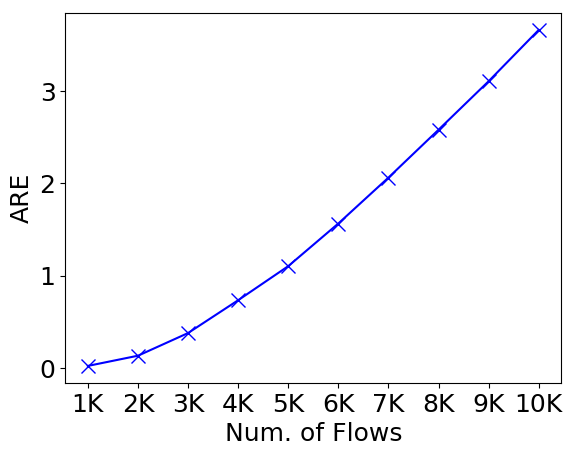
\includegraphics[width=\linewidth]{figures/exp84482/count_min_sketch_are}
        \caption{The average relative error of the count-min sketch as the number of flows increases from 1K to 10K.}
        \label{fig:countminsketchare}
    \end{minipage}
\end{figure}

\subsection{Elephant flows are more important than mice flows.}
Once the memory size is fixed, the number of flows that can be stored without degrading accuracy is fixed too. For most applications such as heavy hitter detection, traffic engineering and ISP billing, elephant flows are more important than small flows. On the contrary, usually it is enough to record the number of mice flows and the total number of packets corresponding to the flows. Moreover, due to the skewed characteristics of the network traffic\cite{benson_network_2010}, the number of mice flows is far greater than that of elephant flows, while the range of flow sizes of elephant flows is much greater than that of mice flows. For example, we define the flows with no less than 10 packets as elephant flows. For the CAIDA trace shown in Table~\ref{tab:netflowtraces},  only 3.1\% of the flows are elephant flows, the sizes of elephant flows have the range of [10, 110900], and 52.9\% of the packets are from the elephant flows. For the campus trace only 7.7\% of the flows are elephant flows while the sizes of elephant flows have the range of [10, 289877] and more than 85\% of the packets are from the elephant flows. So elephant flows are richer in information and it is reasonable to cache the elephant flows preferentially. 


\subsection{It is reasonable to tradeoff computation for higher memory utilization}
\label{subsection:computationmemoryutilizationtradeoff}
The conventional methods for handling collision in hash table such as cuckoo hash\cite{pagh_cuckoo_2004}\cite{chen_dynamic_2017} are infeasible for the scenario of network measurement since they require unlimited memory accesses in the worst case. Inspired by \emph{the power of two choices}\cite{byers_geometric_2004}\cite{doerr_stabilizing_2011}\cite{mitzenmacher_using_2007}\cite{mitzenmacher_power_2001}, we consider using multiple hash functions for handling collisions. When a new flow arrives we map it to the table using the first hash function. If collision occurs we map it using the second hash function. We do this all the way until an empty cell is found. If functions associated with the table are used up and no empty cell is found, the flow is discarded. 

Denote the number of hash functions associated with the table by $d$. Suppose the hash table consists of $n$ cells and we feed $n$ flows into it. The \emph{utilization} of the hash table is defined as $utilization=\frac{m}{n}$, where $m$ is the number of flows cached in the hash table successfully. 

In the case of $d=1$, after inserting $n$ flows, the probability that a given cell of the hash table is empty is 
\begin{equation}\label{key}
p_1 = (1 - \frac{1}{n})^n\approx \frac{1}{e}
\end{equation}

So the number of empty cells  as well as the number of flows that fail to be cached after insertion is $n\times p_1$. The utilization of the hash table is 
\begin{equation}
u_1 = \frac{n-n\times p_1}{n} = 1-p_1 = 1 - \frac{1}{e}
\end{equation}

Now consider the case where $d=2$. Firstly we map the flows to the table using the first function, which is the same as the case where $d=1$. So there will be $n\cdot p_1$ flows that are waiting to be cached using the second hash function. The probability that there is no flows mapped to a given cell during the second run of insertion is
\begin{equation}
(1 - \frac{1}{n})^{n\times p_1}\approx(\frac{1}{e})^{p_1}
\end{equation}

So the probability that a cell is empty after two runs of insertion is :
\begin{equation}
p_2 = p_1\cdot (\frac{1}{e})^{p_1}
\end{equation}
and the utilization of the hash table is:
\begin{equation}
u_2 = \frac{n - n\times p_2}{n} = 1 - p2
\end{equation}

Similarly, the utilization of the hash table when $d=k$ is:
\begin{equation}
u_k = 1 - p_k
\end{equation}
where $p_k$ is the probability that a given cell is empty after $k$ runs of insertion, and $p_1 = \frac{1}{e}$, $p_i = p_{i-1}\cdot (\frac{1}{e})^{p_{i-1}}$ for $i = 2, 3, \cdots, k$.

As shown in Fig.~\ref{fig:cachehitratio}, when we increase the value of $d$ from 1 to 10, the utilization of the hash table increases from 63\% to 92\%. So we can use more hash functions and improve the utilization of memory space by doing more computations.
\fi
